% !TEX root = main.tex

\section{Path explosion}
\label{se:path-explosion}

One of the main challenges of symbolic execution is the path explosion problem. Since symbolic execution may fork off a new execution engine instance at every branch, the total number of executors may be exponential in the number of branches of the program. This impacts both time and space, as a symbolic executor may need to keep track of an exponential number of pending branches to be explore. A common approach is to compute an under-approximation of the analysis that only explores a relevant subset of the state space.
\mynote{I: We could add the following two examples to explain the causes of path explosion (Vechev)}

\iffalse
\begin{itemize}

\item Exponential in branching structure: in the example, 3 variables, 8 paths (can we generalize? $t$ variables, $2^t$ paths?)

\begin{verbatim}
1. int a = ?, b = ?, c = ?; // symbolic
2. if (a) ... else ...;
3. if (b) ... else ...;
4. if (c) ... else ...;
\end{verbatim}

\item Loops on symbolic variables even worse

\begin{verbatim}
1. int a = ?; // symbolic
2. while (a) do ...;
3.
\end{verbatim}
\item Potentially $2^{31}$ paths through loop!

\end{itemize}
\fi

% ---------------------------------------------------------------------------------------------------
\subsection{Pruning Unrealizable Paths}
\label{ss:unrealizable-paths}

A first natural technique for reducing the path space is invoking the constraint solver at each branch, pruning branches that are not realizable. Indeed, if the constraint solver is able to prove that the logical formula given by the path constraints of a branch is not satisfiable, then there exists no assignment of the program input values that would drive a real execution towards that branch. For this reason, the symbolic engine can safely discard the path involving that branch without affecting soundness of the approach. \mynote{E: aggiungiamo un piccolo esempio?}This approach is commonly referred as {\em eager evaluation} of path constraints and is typically the default approach adopted by most symbolic engines. We refer to Section~\ref{ss:constraint-reuse} for a discussion of the possible benefits given by the opposite strategy, i.e., {\em lazy evaluation}.

% From warm-up example\mynote{IF: I removed from the warm up the non-forking case. Must be explained here}:

% The evaluation of a conditional branch ${\tt if}~e~{\tt then}~s_{true}~{\tt else}~s_{false}$ affects the path constraint. Two scenarios are possible:
%     \begin{enumerate}
%       \item {\em Non-forking}: if $e$ is evaluated as always true (resp., false) under the assumptions in the current state, the proper branch is taken and the symbolic execution advances to $s_{true}$ (resp., $s_{false}$);
%       \item {\em Forking}: if $e$ cannot be evaluated without instantiating values for one or more of its symbols, the symbolic execution is forked by creating two execution states with path constraints $pct_{true}$ and $pct_{false}$, respectively, corresponding to the two {\tt if} branches. Namely, $pct_{true}=pct \wedge e_s$ and $pct_{false}=pct \wedge \neg e_s$, where $e_s$ is a symbolic expression obtained by evaluating $e$. 
% %        \[ (s_{true}, pc_{true}) \text{ where } pc_{true} = pc \wedge e \]
% %        \[ (s_{false}, pc_{false}) \text{ where } pc_{false} = pc \wedge \neg e \]
%     Symbolic execution proceeds on both states in parallel.
%     \end{enumerate}


\begin{figure}[t]
  \centering
  \begin{adjustbox}{width=1\columnwidth}
  \begin{small}
  \begin{tabular}{| l || l |}
    \hline      
    {\bf Heuristic} & {\bf Goal} \\ \hline\hline
    BFS & {\em Maximize coverage} \\ & \cite{CKC-TOCS12,PEX-TAP08} \\\hline
    DFS & {\em Exhaust paths, minimize memory usage} \\ & \cite{EXE-CCS06,CKC-TOCS12,PEX-TAP08,DART-PLDI05} \\\hline
    Random path selection & {\em Randomly pick a path with probability based on its length} \\ & \cite{KLEE-OSDI08} \\\hline
    %low-covered code & prioritize paths that execute low-covered code  & \cite{EXE-CCS06} \\
    Code coverage search & {\em Prioritize paths that may explore unexplored code} \\ & \cite{EXE-CCS06,KLEE-OSDI08,MAYHEM-SP12,CKC-TOCS12,GV-ISSTA02} \\\hline
    Buggy-path-first & {\em Prioritize bug-friendly path} \\ & \cite{AEG-NDSS11} \\\hline
    Loop exhaustion & {\em Fully explore specific loops} \\ & \cite{AEG-NDSS11} \\\hline
    Symbolic instruction pointers & {\em Prioritize paths with symbolic instruction pointers} \\ & \cite{MAYHEM-SP12} \\\hline
    Symbolic memory accesses & {\em Prioritize paths with symbolic memory accesses} \\ & \cite{MAYHEM-SP12} \\ \hline
    Fitness function & {\em Prioritize paths based on a fitness function} \\ & \cite{XTD-DSN09,CS-CACM13,XTD-DSN09} \\ \hline
    Subpath-guided search & {\em Use frequency distributions of explored subpaths to prioritize less covered parts of a program} \\ & \cite{LZL-OOPSLA13} \\
    %kill path & filter uninteresting path & \cite{CKC-TOCS12} \\
    \hline  
  \end{tabular}
  \end{small}
  \end{adjustbox}
  \caption{A representative list of path selection heuristics discussed in literature.}
  \label{tab:heuristics}
\end{figure}


% ---------------------------------------------------------------------------------------------------
\subsection{Bounding Computational Resources}
\label{heuristics}

Another common approach is to limit the amount of resources symbolic execution is allowed to use. For instance, the computation may time out after a certain amount of time. Since only a fraction of paths may be explored, the search should be prioritized by looking at the most promising paths first. There are several strategies for selecting or generating the next path to be explored. We now briefly overview some of the most interesting techniques that have been shown to be effective in the literature. %in prior works.

\subsubsection{Search Heuristics}
\label{sss:search-heuristics}

% many prior works
Given a set of unexplored paths, a search heuristics should select the most promising path to explore. Many works have introduced novel search strategies, showing their effectiveness in specific application contexts. These heuristics have often been tailored to help the symbolic engine achieve a specific goal (e.g., overflow detection). Finding a universally optimal strategy for prioritizing path exploration remains an open problem. Table~\ref{tab:heuristics} provides a sample of the most interesting search heuristics discussed in prior works. 

The most common strategies are {\em depth-first search} (DFS) and {\em breadth-first search} (BFS). DFS continuously expands a path as much as possible, before backtracking to the last unexplored branch. BFS explores all unexplored paths in parallel, repeatedly expanding each of them by a fixed slice. DFS is often adopted for minimizing the memory usage of the symbolic engine: since the chosen path will be sooner or later fully explored, the memory needed for keeping its state will be released as well. Unfortunately, paths containing loops and recursive calls can easily stall the symbolic engine. For this reason, some tools prefer prioritizing paths using BFS. Although memory pressure can be higher, this strategy may allow an engine to quickly explore diverse paths and possibly detecting interesting behaviors. On the other hand, if the ultimate goal requires to fully terminate the exploration of one or more paths, BFS may take a very long time.

Another very popular strategy is {\em random path selection} that, as its name would suggest, randomly picks a path for exploration. This heuristic has been refined in several variants. For instance, {\sc KLEE}~\cite{KLEE-OSDI08} assigns probabilities to paths based on their length and on the branch arity. Namely, it favors paths that have been explored fewer times, preventing starvation caused by loops and other path explosion factors.

% have instead presented
Several works, such as {\sc EXE}~\cite{EXE-CCS06}, {\sc KLEE}~\cite{KLEE-OSDI08}, {\sc Mayhem}~\cite{MAYHEM-SP12}, and {\sc \stwoe}~\cite{CKC-TOCS12}, have discussed heuristics aimed at maximizing code coverage. For instance, the {\em coverage optimize search} discussed in {\sc KLEE}~\cite{KLEE-OSDI08} computes a weight for each state and then randomly selects a state according to these weights. The weight is obtained by taking into account the minimum distance to an uncovered instruction, the call stack of the state, and whether the state has recently covered new code. Of a similar flavor is the heuristic proposed in~\cite{LZL-OOPSLA13}, called {\em subpath-guided search}, that attempts to explore {\it less traveled} parts of a program by selecting the subpath that have been explored fewer times. This is achieved by maintaining a frequency distribution of explored subpaths, where a subpath is defined as a postfix of length $n$ of a path. Interestingly, the value $n$ plays a crucial role with respect to code coverage achieved by a symbolic engine exploiting this heuristic and no specific value has been shown to be universally optimal.

Other search heuristics try to prioritize paths likely leading to states that are {\em interesting} according to some goal. For instance, the {\em buggy-path first} strategy in {\sc AEG}~\cite{AEG-NDSS11} picks paths whose past states have contained small but unexploitable bugs. The intuition is that if a path contains some small errors, it is likely that it has not been properly tested. There is thus a good chance that future states may contain interesting, and hopefully exploitable, bugs. Similarly, the {\em loop exhaustion} strategy discussed in {\sc AEG}~\cite{AEG-NDSS11} explores paths that are visiting loops. This approach is inspired by the practical observation that common programming mistakes in loops may lead to buffer overflows or to other memory-related errors. In order to find exploitable bugs, {\sc Mayhem}~\cite{MAYHEM-SP12} instead gives priority to paths where symbolic memory accesses are identified or symbolic instruction pointers are detected. 

Fitness functions have been extensively used in the context of search-based test generation~\cite{M-STVR04}. \mynote{[D] Check and rephrase 2nd sentence}A fitness function measures how close an explored path is to achieve the target test coverage. Several papers, e.g.,~\cite{XTD-DSN09,CS-CACM13,XTD-DSN09}, have applied this idea in the context of symbolic execution. As an example,~\cite{XTD-DSN09} introduces {\em fitnex}, a strategy for concolic execution that prioritizes paths that are {\em closer} to take a specific branch. In more detail, given a branch condition of the form $|a - c| == 0$ and a path that has reached the branch, {\em fitnex} computes a closeness equal to $|a - c|$ by leveraging the concrete values of two variables $a$ and $c$ in that path. Similar fitness values can be computed for other kinds of branch conditions. The path with the lowest fitness value for a branch is selected by the symbolic engine. Paths that have not yet reached the branch get the worst-case fitness value.

\begin{comment}
\begin{itemize}

  \item \cite{AEG-NDSS11}:
  \begin{itemize}
    \item {\em buggy-path-first}: priority to path that shown to contain errors (even if not exploitable)
    \item {\em loop exhaustion}: give priority to path that are exhausting a loop. In practice this can hit exploitable bugs (buffer overflows), but can prevent progress. Allow only one executor that is exhausting a loop, perform aggressive preconditioned symbolic execution.
  \end{itemize}

  \item {\em less covered code}: \cite{EXE-CCS06} uses a mixture of best-first and depth-first search. Best-first approach uses heuristic that give high priority to the path which is blocked at the line that has been executed the fewest number of times. The picked path is executed with DFS for a limited amount of time in order to avoid starvation. 

  \item \cite{KLEE-OSDI08} interleaves in a round robin fashion these strategies:
  \begin{itemize}
    \item {\em random path selection}: build a binary tree structure of all the state (each state is always created due to a fork from a parent). Assign same probability of being executed among states of the same subtree. Avoid starvation by given priority to states high in the tree.
    \item {\em coverage optimize search}: assign weights based on how much new code has been covered by a path. Pick up state randomly using weights as probability.
  \end{itemize}
  Each state is executed only for a time slice defined both as maximum number of instructions and as maximum amount of time.

  \item \cite{SAGE-NDSS08}:

  \item \cite{MAYHEM-SP12} same heuristics as~\cite{SAGE-NDSS08} and~\cite{KLEE-OSDI08}:
  \begin{itemize}
    \item executors exploring new code have high priority
    \item executors that identify symbolic memory accesses have high priority
    \item executors where symbolic instruction pointers are detected have high priority
  \end{itemize}

  \item \cite{CS-CACM13} mentions that a {\em fitness function} can be used to drive exploration of input space. Some examples: \cite{BHH-ASE11,LMH-JSS10}.

  \item Priority-based selection in~\cite{CKC-TOCS12}:
    \begin{itemize}
      \item bread-first search
      \item depth-first search
      \item max coverage heuristic
      \item path killer heuristic: kill paths that are no longer of interest (e.g., kill path that repeats sequence of program counters more than $n$ times)
    \end{itemize}

\end{itemize}
\end{comment}

\subsubsection{Dynamic Test Generation}
%\subsubsection{Generational Search}
Traditional symbolic execution does not scale over large programs. Although search heuristics may help prioritize some interesting paths, the symbolic execution may still proceed extremely slow. Indeed, the engine must simulate any instruction of the program and heavily relies on the constraint solver in order to make any progress in the execution. {\em Dynamic test generation}, initially introduced in {\sc DART}~\cite{DART-PLDI05}, is a technique that can help symbolic execution scale over large programs. The main idea is to execute both concretely and symbolically a program. This kind of execution is often referred to as concolic execution (Section~\ref{ss:concrete-concolic-symbolic}). Initially, a random input is generated and a concrete execution is started. In parallel, a symbolic execution is also started. Whenever the concrete execute takes a branch, the symbolic execution is directed toward the same branch and the constraints extracted from the branch condition are added to the current set of path constraints. In other words, the symbolic execution is driven by a specific concrete execution. A consequence of this approach is that the symbolic engine does not need to invoke the constraint solver to decide whether a branch condition is (un)satisfiable, since this is directly tested by the concrete execution. Other paths of the program execution can be then explored by selecting a previously taken branch and by negating its constraints. Using a constraint solver, the symbolic engine can generate a new (random) input that drives the concrete execution toward a new path. This strategy can be repeated as much as needed to achieve the desired coverage.

\begin{figure}[t]
  %\vspace{-3mm}
  %\centering
  \begin{subfigure}{.29\textwidth}
    \vspace{5mm}
    \begin{lstlisting}[basicstyle=\ttfamily\scriptsize]
int bar(int x, int y) {
  if (x < 5 && y >= 6) 
    if (x > 1) return 1;
    else return 2;
  else return 3;
}
    \end{lstlisting}
    \vspace{5mm}
    \caption{}
  \end{subfigure}%
  \hspace{-2mm}
  \begin{subfigure}{.37\textwidth}
    \centering
    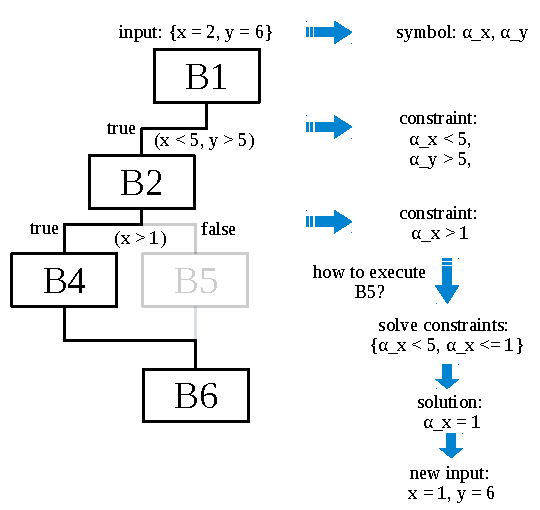
\includegraphics[width=1.0\columnwidth]{images/concolic-execution} 
    %\label{fig:sub1}
    \caption{}
  \end{subfigure}%
  \hspace{-2mm}
  \begin{subfigure}{.33\textwidth}
    \centering
    \vspace{0.05mm}
    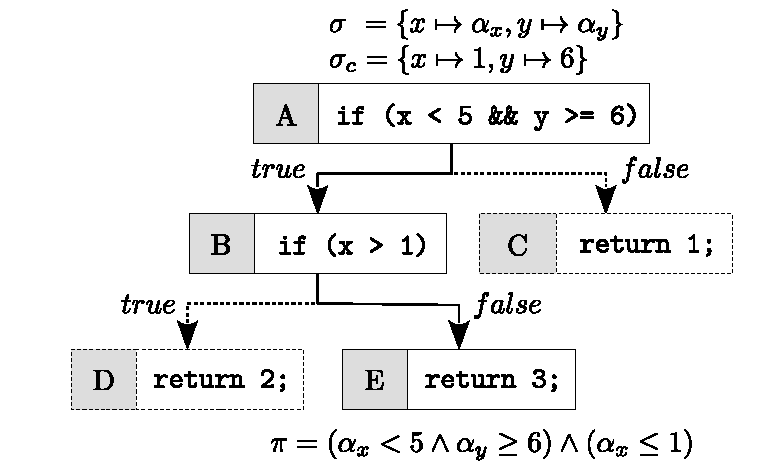
\includegraphics[width=1.1\columnwidth]{images/concolic-execution-2} 
    %\label{fig:sub2}
    \caption{}
  \end{subfigure}
  \caption{(a) Source code of function {\tt bar}. (b) Execution tree for the function {\tt bar}. Solid edges show the path taken by the concolic execution when {\tt x = 2} and {\tt y = 6}. These input values have been randomly chosen. (c) Concolic execution when {\tt x = 1} and {\tt y = 6}. These input values have been obtained using a constraint solver, after negating the path constraints of node B in the function {\tt bar}.}
  \label{fig:example-concrete-execution}
  \vspace{-3mm}
\end{figure}

% pick the values {\tt x = 2} and {\tt y = 6}, respectively
An example of dynamic test generation is shown in Figure~\ref{fig:example-concrete-execution}. Consider the function {\tt bar} (Figure~\ref{fig:example-concrete-execution}a) that takes two integer inputs {\tt x} and {\tt y}. To start a first concrete execution, a symbolic engine may initially randomly pick {\tt x = 2} and {\tt y = 6} as input values. The concrete execution induced by these inputs is presented in Figure~\ref{fig:example-concrete-execution}b: both the first (node A) and second branch condition (node B) are satisfied, directing the execution towards the first {\tt return} statement (node D). Other nodes, such as C and E are skipped since their associated branch conditions are not met by the current input values. For instance, node $E$ is not executed since the condition $x > 1$ (node B) directs the path towards the node $D$. An engine that desires to symbolically execute a path containing the node $E$ must track the constraints during the concrete execution over {\tt x = 2} and {\tt y = 6} and then negate the branch condition $x > 1$. To generate a new (random) input, the engine can then invoke a solver over the constraints $\neg(\alpha_x > 1) \wedge (\alpha_x < 5 \wedge \alpha_y > 5)$, possibly getting a valid solution. In our example (Figure~\ref{fig:example-concrete-execution}c), {\tt x = 1} and {\tt y = 6} are the chosen input values by the constrain solver. Notice that since {\tt y} is not involved in the branch condition that is currently negated, the engine may even reuse its value and include an additional constraint $\alpha_y = 6$. This optimization may drastically reduce the solving time required for obtaining a solution from the constraint solver.

Although dynamic test generation uses concrete inputs to drive the symbolic execution toward a specific path, it still needs to pick a branch to negate whenever a new path have to be explored. Notice that each concrete execution may add new branches that still needs to be visited. Since the set of non-taken branches across all the performed concrete executions can be very large, the search heuristics discussed in Section~\ref{heuristics} still play a crucial role. For instance, {\sc DART}~\cite{DART-PLDI05} choses the next branch to negate using a depth-first strategy. Additional strategies for picking the next branch to negate have been presented in literature. For instance, the {\em generational search} algorithm discussed in {\sc SAGE}~\cite{SAGE-NDSS08} systematically yet partially explores the state space, maximizing the number of new tests generated while also avoiding redundancies in the search. This is achieved by negating constraints following a specific order and by limiting the backtracking of the search algorithm.

%\mynote{Add paper on hybrid concolic testing}In particular,



% ---------------------------------------------------------------------------------------------------
\subsection{Preconditioned Symbolic Execution}\mynote{[D] Entirely rewritten}
\label{precontioned-symbolic-execution}

{\sc AEG}~\cite{AEG-NDSS11} proposes {\em preconditional symbolic execution} as a novel method to target symbolic execution towards certain subsets of the input state space. The state space subset is determined by the precondition predicate $\Pi_{prec}$: inputs that do not satisfy $\Pi_{prec}$ will not be explored. The intuition for preconditioned symbolic execution is that we can narrow down the state space we are exploring by specifying exploitability conditions as a precondition, e.g., all symbolic inputs should have the maximum size to trigger buffer overflow bugs. The main benefit of preconditioned symbolic execution is simple: by limiting the size of the input state space before symbolic execution begins, we can prune program paths and therefore explore the target program more efficiently.
Note that preconditions need to be selected carefully. If a precondition is too specific, we will detect no bugs or exploits; if it is too general, we will have to explore almost the entire state space. %Thus, preconditions have to describe common characteristics among exploits (to capture as many as possible) and at the same time it should eliminate a significant portion of non-exploitable inputs.\\
% Note that preconditions cannot be selected at random

% Preconditioned symbolic execution enforces the precondition
This technique enforces a precondition by adding the precondition constraints to the path predicate during initialization. Adding constraints may seem strange since there are more checks to perform at branch points during symbolic execution. However, the state space shrink caused by the precondition constraints outweighs the decision procedure overhead at branching points. When the precondition for a branch is unsatisfiable, we do not make further checks, nor we fork an execution engine instance for the branch.% We note that while we focus only on exploitable paths, the overall technique is more generally applicable.\\

\paragraph{Preconditions} The authors identify 4 different categories of preconditions:
\begin{itemize}
\item {\em None}: there is no precondition, thus space exploration proceeds as normal;
\item {\em Known length}: symbolic inputs are of known maximum length, e.g., a network packet has a fixed size, or static analysis can determine the input length;
%Static analysis techniques can be used to automatically determine this precondition.
\item {\em Known prefix}: symbolic inputs have a known prefix, e.g., a fixed header string such as the initial {\em magic code} in a binary, or a network packet header.
\item {\em Fully known}: all input bytes are concrete, as in a concolic execution; it can be used, for instance, to generate a working exploit from a known crashing input. 
\end{itemize}

\begin{figure}[!ht]
\begin{small}
\begin{lstlisting}[basicstyle=\ttfamily\small]
    // N symbolic branches 
    if (input[0] < 42) [...]
    [...]
    if (input[N-1] < 42) [...]

    // symbolic loop
    strcpy(dest, input); 

    // M symbolic branches
    if (input[N] < 42) [...]
    [...]
    if (input[N+M-1] < 42) [...]
\end{lstlisting}
\end{small}
\caption{\label{fig:preconditioned} Advantages of preconditioned symbolic execution - taken from~{\sc AEG}~\protect\cite{AEG-NDSS11}.}
\end{figure}

\paragraph{Example} Consider the example in Figure~\ref{fig:preconditioned} where {\tt input} is an array of $S\ge N+M$ bytes. The impact of preconditions on the state space size is as follows:


\begin{itemize}
  \item {\em None}: the input space size is $256^S$, and up to $2^N\cdot S\cdot 2^M$ execution engine instances are needed, due to $N+M$ symbolic branches and up to $S$ loop iterations;
  \item {\em Known length}: if we assume a string length $S$, i.e., the first $(S-1)$ bytes of {\tt input} are not $\setminus0$, the loop is concretized, and the state space size is reduced to $2^{N+M}$;
  \item {\em Known prefix}: if a prefix of $P<N$ bytes is known for {\tt input}, the first $P$ branches and $P$ loop iterations are concrete, and the state space size becomes $2^{N-P}\cdot S\cdot 2^M$;
  \item {\em Fully known}: as all input bytes are concrete, the state space size is trivially $1$.
\end{itemize}

% [D] shall we mention that for prefixes also inequalities can be used, and that prefixes while they reduce the space size, they can lead to missing interesting states, e.g., malformed headers? I think it would be a bit too much detailed


% ---------------------------------------------------------------------------------------------------

%\subsection{Dynamic symbolic execution}
%Dynamic symbolic execution refers to a body of techniques that exploit execution with concrete values to explore [...].

% ---------------------------------------------------------------------------------------------------
\subsection{Under-constrained Symbolic Execution} 
\label{under-constrained}

A possible approach to avoid path explosion is to cut the code to check, say a function, out of its encolosing system and check it in isolation. Lazy initialization with user-specified preconditions (Section~\ref{ss:complex-objects}) follows this principle in order to automatically reconstruct complex  data structures. However, cutting a code region out of an application has proven to be quite difficult due to the entanglements with the surrounding environment~\cite{ED-ISSTA07}.

% certain values (e.g., a null pointer)
Indeed, errors detected in a function analyzed in isolation may be false positives, as the input may never assume certain values when the function is executed in the context of a full program. Some prior works, e.g., {\sc Check 'n' Crash}~\cite{CS-ICSE05}, first analyze the code in isolation and then test the generated crashing inputs using concrete executions.

{\em Under-constrained symbolic execution}~\cite{ED-ISSTA07} is a twist on symbolic execution that allows for the analysis of a function in isolation by marking symbolic inputs for which preconditions are missing as {\em under-constrained}. Intuitively, missing preconditions are the constraints on the variable yielded along the path prefix from the program's entry point to the function. Under-constrained variables have the same semantics as classic symbolic variables except when used in an expression that can cause an error to occur. In this case, an error is reported only if all the solutions for the currently known constraints on the variable cause it to occur, i.e., the error is context-insensitive and a true positive. Otherwise, its negation is added to the path constraints and execution resumes as normal. This choice can be regarded as an attempt to reconstruct preconditions from the checks inserted in the code. Any subsequent action violating an added negated constraint will be reported as an error.

Although this technique is not sound as it may miss errors, it can still scale to find interesting bugs in larger programs. Also, the application of under-constrained symbolic execution is not limited to functions only: for instance, if a code region (e.g., a loop) may be troublesome for the symbolic executor, it can be skipped by marking the locations affected by it as under-constrained.


\iffalse % [D] original text here, while commented text has been moved to sandbox.tex
%By isolating a function from the rest of the program, we can perform symbolic execution on it.
A possible approach to avoid path explosion with function calls is to symbolically execute a function in isolation. The results of the analysis can then be exploited when any other code region is symbolically executed and a call to the function is present. However, errors detected in the isolated function may be false positives since the input may never assume certain values (e.g., a null pointer) when the function is executed in the context of the full program. Some prior works, e.g., \cite{CS-ICSE05}\mynote{check this paper}, first analyze the code in isolation and then test the generated crashing inputs using concrete executions. % However, errors detected in the isolated function may be false positives since some of the input values may never been valid when the function is actually executed in the context of the full program

{\em Under-constrained symbolic execution}~\cite{ED-ISSTA07} is a technique that performs symbolic execution of an isolated function and explicitly marks which symbols are {\em under-constrained} (i.e., their symbolic values might violate preconditions due to missing constraints) to distinguish them from {\em exactly constrained} symbols.

Errors due to concrete values and exactly constrained symbols are treated as true positives. On the other hand, errors due to under-constraining are treated as true positives only if {\em all} the solutions to the currently known constraints on the symbols cause the error to occur. Otherwise the negation of the error is added to the constraint set and the symbolic execution of the isolated function is continued. In other words, an error is \mynote{[D] added promptly} promptly reported if and only if it is {\em context-insensitive}. Notice that a symbol may initially be under-constrained and then become exactly constrained. For instance, consider the following piece of code:

    \begin{lstlisting}[basicstyle=\ttfamily\small]
    assert(a != 0); // no knowledge about a
    a = 0;          // from now on a's value is known
    assert(a != 0); // error always hits: context-insensitive! 
    \end{lstlisting}

If {\tt a} is marked as under-constrained, then the first {\tt assert} will not trigger an error: indeed, there is at least one possible value for the symbol associated to {\tt a} that does not hit the error. Conversely, the second {\tt assert} will always trigger an error since {\tt a} has a concrete value and is not under-constrained anymore.

Although this technique is not able to find {\em all} the possible errors in a function, it can still find interesting bugs. Moreover, since symbolically executing a whole program may be unfeasible, this technique allows for testing a large number of lines of code in a reasonable amount of time. In particular, this technique allows an engine to skip code: if a function or any other construct (e.g., a loop) may be troublesome for symbolic execution, it can be skipped by just marking the locations affected by it as under-constrained. However, a possible implementation issue is given by the propagation of under-constrained symbols: given an instruction of the form {\tt if (s < t)}, if {\tt t} is under-constrained while {\tt s} is exactly constrained then when the symbolic execution proceeds through the two possible branches, {\tt s} must be marked as under-constrained. Some optimizations may thus be needed in order to minimize this propagation effect.
\fi

% ---------------------------------------------------------------------------------------------------
\subsection{State Merging}

Several static program analysis techniques such as abstract interpretation merge states corresponding to different paths into a state that over-approximates them. In a precise symbolic execution, however, merging is not allowed to introduce any approximation or abstraction, and therefore can only change formulas to have them characterize sets of execution paths. In other words, a merged state will be described by a formula that represents the disjunction of the formulas that would have described the individual states if they were kept separate.

\paragraph{Example} Consider the following piece of code:
    \begin{lstlisting}[basicstyle=\ttfamily\small]
    1.  void foo(int x, int y) {
    2.    if (x < 5)
    3.      y = y * 2;
    4.    else
    5.      y = y * 3;
    6.    return y;
    7.  }
    \end{lstlisting}
The symbolic execution of this function is shown in Figure~\ref{fig:example-state-merging}a. Initially (execution state $A$) the path constraints are {\tt true} and input arguments {\tt x} and {\tt y} are associated with symbolic values $\alpha_x$ and $\alpha_y$, respectively. Line 2 contains a conditional branch and the execution is forked: depending on the branch taken, a different statement is evaluated next and different assumptions are made on symbol $\alpha_x$ (execution states $C$ and $D$, respectively). After expanding every execution state until the {\tt return} at line 6 is reached on all branches, the symbolic execution gets populated with two additional execution states D and E. If a symbolic execution engine desires to reduce the number of active states, then state merging can be performed. For instance, Figure~\ref{fig:example-state-merging}b shows the symbolic execution tree for the same piece of code when a state merging operation is performed before evaluating the {\tt return} statement at line 6: D$'$ is now a merged state that fully captures the former execution states D and E. Indeed, the $ite(\texttt{c}, \texttt{t}, \texttt{f})$ expression introduced in the symbolic store $\sigma$ is a short term for an {\tt if-then-else} expression and means that if the condition {\tt c} is verified then {\tt t} holds, otherwise {\tt f} must be assumed as true. Nonetheless, $ite$ expressions are often just syntactic sugar for disjunctive formulas and are commonly supported by most prominent constraint solvers. For instance, in the context of propositional logic the $ite(\texttt{c}, \texttt{t}, \texttt{f})$  expression could be replaced with the formula $(\texttt{c} \wedge \texttt{t}) \vee (\neg\texttt{c} \wedge \texttt{f})$ . However, since the symbolic store in our model should return an integer value for variable $y$ rather than a boolean value, following the idea presented in~\cite{KP-PP05}, the $ite$ expression could be translated into the expression $((\alpha_x < 5) * (2 * \alpha_y)) + (\neg(\alpha_x < 5) * (3 * \alpha_y))$ that evaluates\footnote{We are assuming that the result of a comparison maps to integer values 0 or 1.} to the actual value of {\tt y} based on the branch condition at line 2. Indeed, the condition $(\alpha_x < 5)$ could be either true or false, yielding to only one of two possible values of $y$. On the other hand, the path constraints of the execution states C and D has been just merged into the disjunction formula $\alpha_x < 5 \vee \alpha_x \geq 5$ and then simplified to $true$ value.

%$(\alpha_x < 5 \wedge 2 * \alpha_y) \vee (\neg(\alpha_x < 5) \wedge 3 * \alpha_y)$



% Constructing Efficient Formal Models from High-Level Descriptions Using Symbolic Simulation

%As depicted by the symbolic execution tree shown in Figure~\ref{fig:example-state-merging}, when {\tt foo} is symbolically executed, the two input parameters {\tt x} and {\tt y} are mapped to the symbols  Whenever the branch condition on line 2 is evaluated, the two parallel execution states B and C are generated. Accordingly to taken branch, a different line of code is then evaluated, leading to execution states D and E. 


%In the branch where $\alpha_a\neq 0$, variable {\tt y} is assigned with ${\tt x}+3$, obtaining $y\mapsto 4$ in state $E$ because $x\mapsto 1$ in state $C$. In general, arithmetic expression evaluation simply manipulates the symbolic values.

%\noindent A symbolic execution engine may perform state merging in the following way:\noindent where {\em ite} represents an {\tt if-then-else} statement and $\bot$ a non-taken branch.

\begin{figure}[t]
  \vspace{-3mm}
  \centering
  \begin{subfigure}{.5\textwidth}
    \centering
    \hspace{-5mm}
    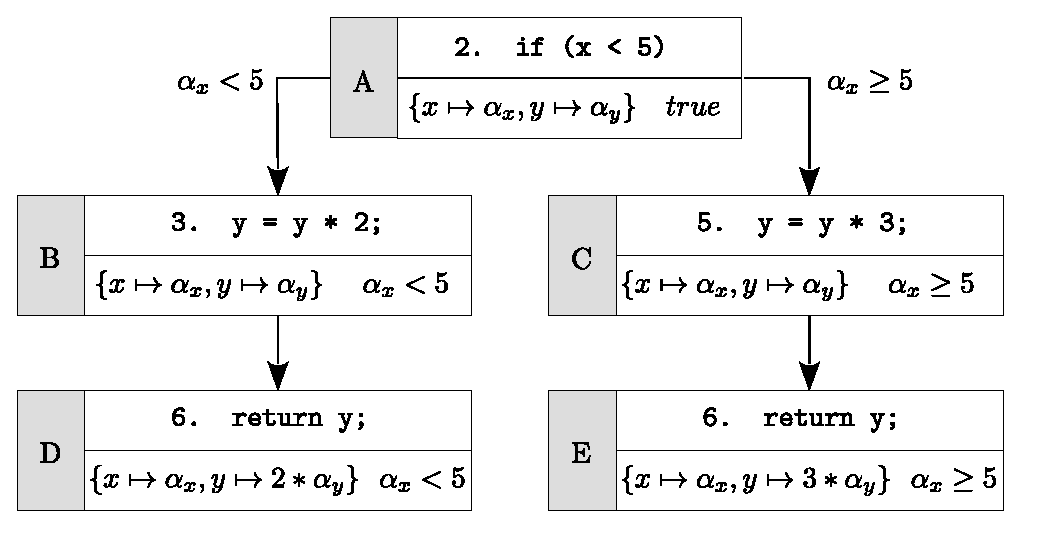
\includegraphics[width=1.05\columnwidth]{images/state-merging} 
    %\label{fig:sub1}
    \caption{}
  \end{subfigure}%
  \begin{subfigure}{.5\textwidth}
    \centering
    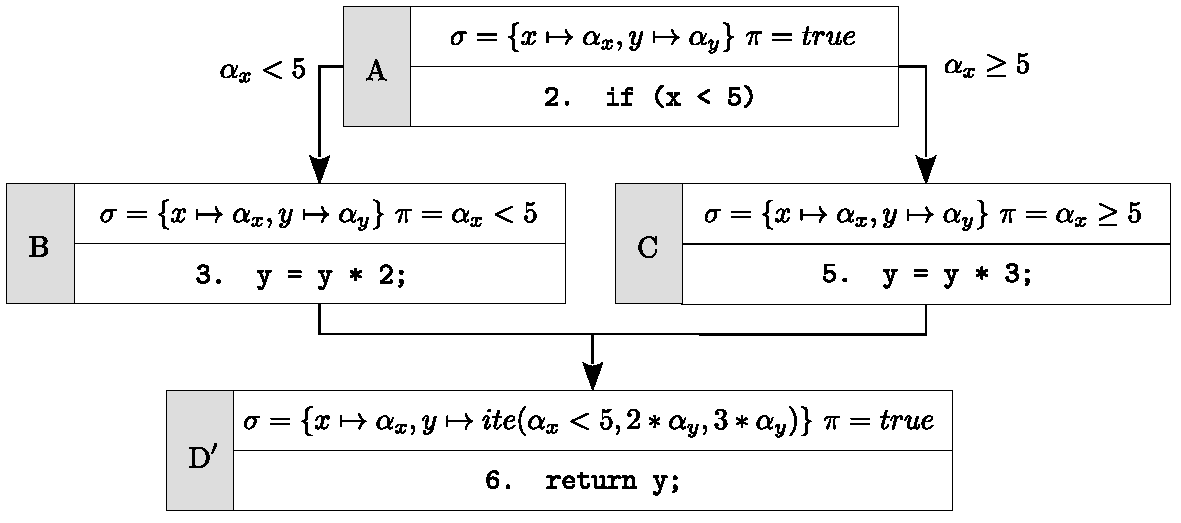
\includegraphics[width=1.05\columnwidth]{images/state-merging-2} 
    %\label{fig:sub2}
    \caption{}
  \end{subfigure}
  \caption{(a) Symbolic execution tree of the function {\tt foo} without state merging; (b) Symbolic execution DAG of the function {\tt foo} with state merging.}
  \label{fig:example-state-merging}
\end{figure}


\paragraph{Trade-off} Early works~\cite{G-POPL07,HSS-RV09} have shown that merging techniques effectively decrease the number of paths to explore, but also put a burden on constraints solvers, which typically encounter difficulties when dealing with disjunction. Merging can also introduce new symbolic expressions in the code, for instance when merging different concrete values from a conditional assignment into a symbolic expression over the condition. \cite{KKB-PLDI12} provides an excellent discussion of the design space of state merging techniques. At one end of the spectrum, complete separation of the paths does not perform any merge and is used in search-based symbolic execution (Section~\ref{sss:search-heuristics}). At the other end, static state merging combines states at control-flow join points, thus essentially representing a whole program with a single formula. Static state merging is used in whole-program verification condition generators, e.g, ~\cite{SATURN-POPL05,CALYSTO-ICSE08}), which typically trade precision for scalability by, for instance, unrolling loops only once.

%At the other end, static state merging combines states at control-flow join points after all subpaths leading to a join point have been explored.

\mynote{Function summaries}

\paragraph{Merging heuristics} Intermediate merging solutions adopt heuristics to identify state merges that can speed the exploration process up. Indeed, generating larger symbolic expressions and possibly extra solvers invocations can outweigh the benefit of having fewer states, leading to poorer overall performance~\cite{HSS-RV09,KKB-PLDI12}. {\em Query count estimation}~\cite{KKB-PLDI12} relies on a simple static analysis to identify how often each variable is used in branch conditions past any given point in the CFG. The estimate is used as a proxy for the number of solver queries that a given variable is likely to be part of. Two states make a good candidate for merging when their differing variables are expected to appear infrequently in later queries. {\em Veritesting}~\cite{VERITESTING-ICSE14} identifies sequences of statements that do not contain system calls, indirect jumps, and other statements that are difficult to reason about statically, and represents them with a single formula as in static state merging. The approach is alternated with a per-path basis symbolic exploration every time a hard-to-analyze statement is encountered. 

\paragraph{State space exploration} In order to maximize the opportunities for merging a symbolic execution engine should traverse a CFG in a topological order, so that a combined state for a program point can be computed from its predecessors. However, this would prevent search exploration strategies aiming at prioritizing more ``interesting'' states over others. ~\cite{KKB-PLDI12} introduces {\em dynamic state merging} to identify opportunities for merging regardless of the exploration order imposed by the search strategy.
Suppose the symbolic engine maintains a worklist of states and a bounded history of their predecessors. When the engine has to pick the next state to explore, it will first check whether there are two states $s_1$ and $s_2$ from the worklist such that they do not match for merging, but $s_1$ and a predecessor $\text{s}^{\prime}_2$ of $s_2$ do. If the expected similarity between $s_2$ and a successor of $s_1$ is high, the algorithm will attempt a merge by advancing the execution of $s_1$ for a fixed number of steps. This capture the idea that if two states are similar, then also their respective successors are likely to become similar in a few steps. If the merge fails, the algorithm will let the search heuristic pick the next state to explore.

%This is useful, for instance, for unbounded loops for which search-based symbolic execution engines would employ search strategies that prioritize exploring new code over unrolling, while static state merging would require a depth-first exploration and thus fully unroll the possibly infinitely many iterations of the loop.

% ---------------------------------------------------------------------------------------------------
\subsection{Limiting State Space through other Program Analysis Techniques}

Other static or dynamic techniques can be used to help a symbolic engine to focus on interesting states:
\begin{itemize}
  \item {\em program slicing} is a method that starting from a subset of a program's behavior, it extracts from the program the minimal sequence of instructions that faithfully represents that behavior~\cite{Weiser84}; we discuss an example of use in Section~\ref{ss:auth-bypass}; 
  \item {\em taint analysis} \mynote{[D] is it accurate to say concolic only?} attempts to identify variables that can be modified by predefined taint sources such as user input and can be performed both statically and dynamically; dynamic taint analysis typically yields more accurate results, and can is often employed in concolic executors to explore symbolically only the parts of an execution that depend upon tainted values~\cite{SAB-SP10};
  \item {\em fuzzing} is a software testing technique that randomly mutates user-provided test inputs to cause crashes or assertion failures and find potential memory leaks; fuzzing can be augmented with symbolic execution to collect contraints for an input and negate them to generate new inputs\footnote{\cite{DRILLER-NDSS16} classifies offline symbolic executors such as {\sc DART} and {\sc SAGE} as whitebox fuzzers.}; on the other hand, a symbolic executor can be augmented with fuzzing to reach deeper states in the exploration more quickly and efficiently: we present two embodiments of this approach in Section~\ref{ss:bug-detection}; 
  \item {\em source code analysis}: extraction of input properties (e.g., size or contents of an array)

  \item {\em phi-node folding} is a code transformation that can be used for statically merging some paths\mynote{E: relation with state merging?}. The main idea is to replace branches with predicated select instructions. Using this technique, the number of paths that must be explored by a symbolic engine can be significantly decreased. For instance,~\cite{CCK-EUROSYS11} used an aggressive variant of phi-node folding, called {\em if-conversion}~\cite{CCF-CGO03}, that allowed them to reduce the number of paths by an exponential factor on some benchmarks.

  %\item {\em compositional techniques}: caching and reusing the analysis of lower-level function in subsequent computations. The main idea is to compute function summaries. See, e.g.,~\cite{G-POPL07,G-PLDI11,MS-TR07}.
  \item {\em abstraction}~\cite{C-SEFM07} is a technique that may be used for computing {\em under-approximations} or {\em over-approximations} of a program state. This approach has been exploited in prior works~\cite{APV-SPIN06,VPP-ISSTA06,XGM-ISSTA08}\mynote{check these papers}. Since some of these works reason about state subsumption, they may be connected with the incremental solving optimization discussed in Section~\ref{constraint-optimizations}.
  \item {\em type-checking}: \cite{KCF-PLDI10} shows how symbolic analysis can be effectively mixed with type-checking analysis. For instance, type-checking analysis can help a symbolic execution engine by detecting the type of an object (e.g., the type of a value returned by a {\em hard to reason} function). Although no assumption can be made on the value of the returned type, this information may still be useful for the symbolic engine (e.g., if the type has a fixed size, some preconditions can be set, possibly pruning some paths). Similarly, symbolic analysis can help a type checker. For instance, the symbolic engine may provide context-sensitive properties over a variable that clearly rules out type errors, reducing the number of false positive given by a traditional context-insensitive type checker.
%\item \cite{DRILLER-NDSS16} is an example of {\em symbolic-assisted fuzzing}: their technique temporarily exploits concolic execution only when a fuzzer cannot generate a valid input to explore an uncovered branch.
\end{itemize}

